\section{Appendices}
\label{sec:appendices}
\subsection{Magnetic field calibration}
		
		\begin{figure}[h]
		    \centering
		    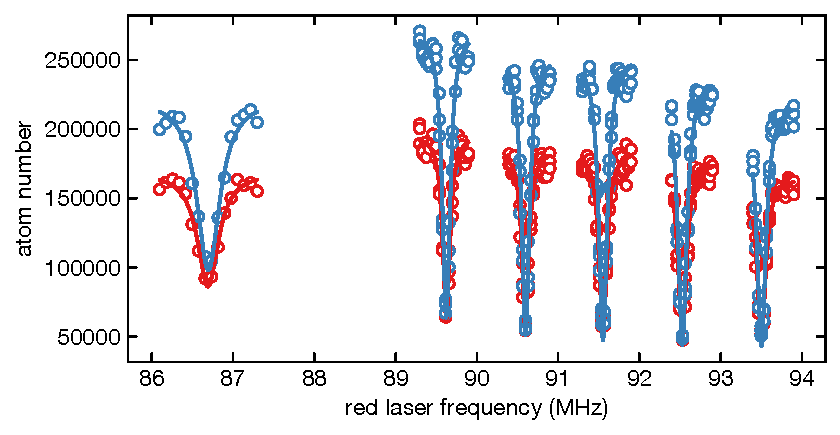
\includegraphics[scale=0.8]{figures/field_calibration.pdf}
		    \caption{\TPO m=1 transition frequency shift as a function of field set voltage datapath:\textbackslash data \textbackslash\_2020\textbackslash10\textbackslash26\textbackslash it\_field\_calibration}
		    \label{fig:field_calibration}
		\end{figure}

		\begin{figure}
		    \centering
		    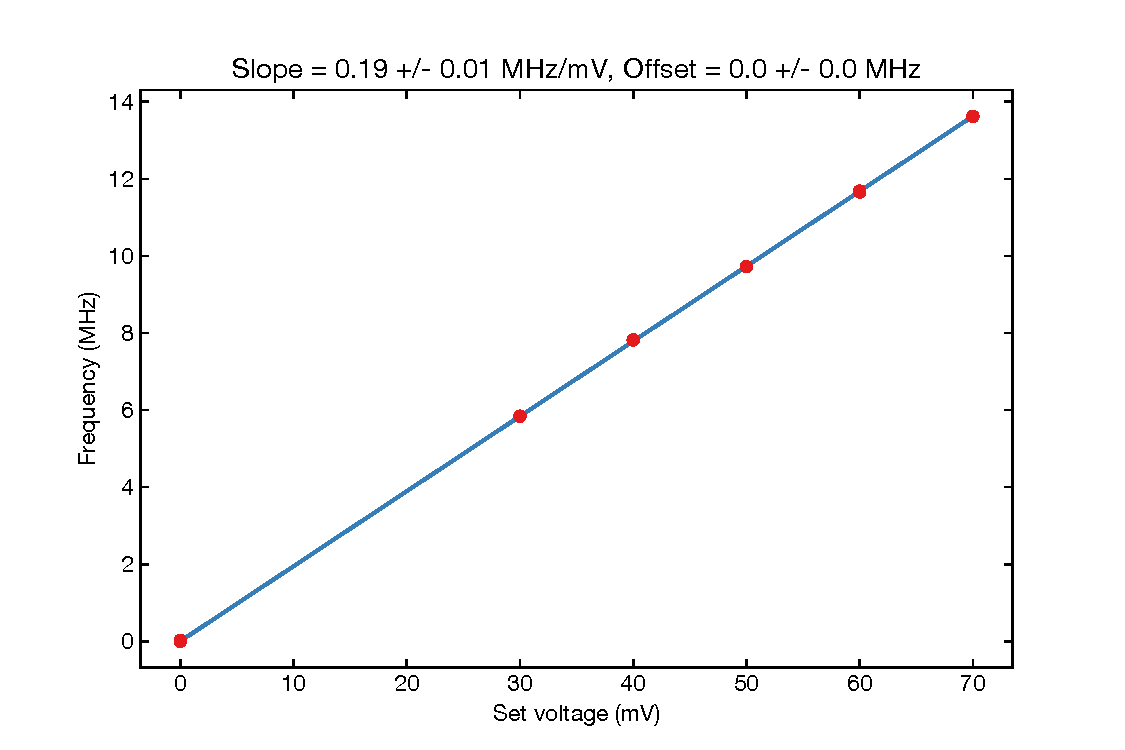
\includegraphics[scale=0.8]{figures/field_calib_curve.pdf}
		    \caption{field calibration curve}
		    \label{fig:field_calib_curve}
		\end{figure}

\subsection{Clock laser waist calibration}
\subsection{Quadratic Zeeman Shift}

		\begin{figure}
		\centering
		\label{fig:qz}
		\begin{subfigure}{0.4\linewidth}
		    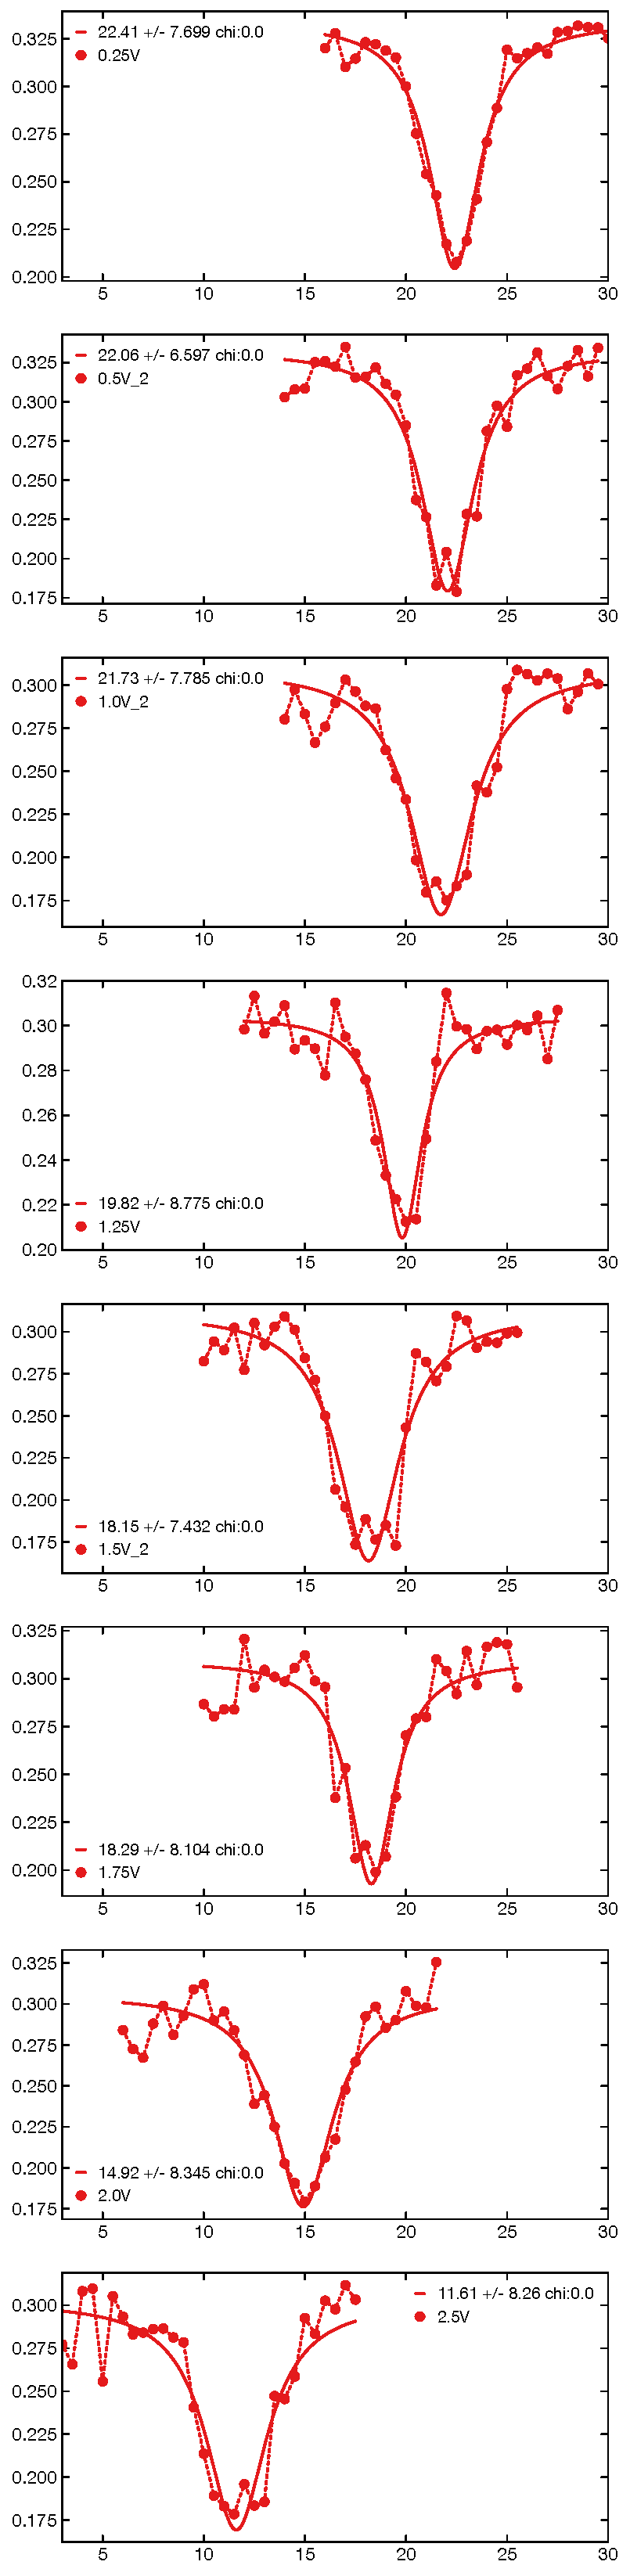
\includegraphics[scale=0.4]{figures/qz_spectrum.pdf}
		    \caption{clock resonant frequency shift for different field}
		\end{subfigure}
		\begin{subfigure}{0.4\linewidth}
		    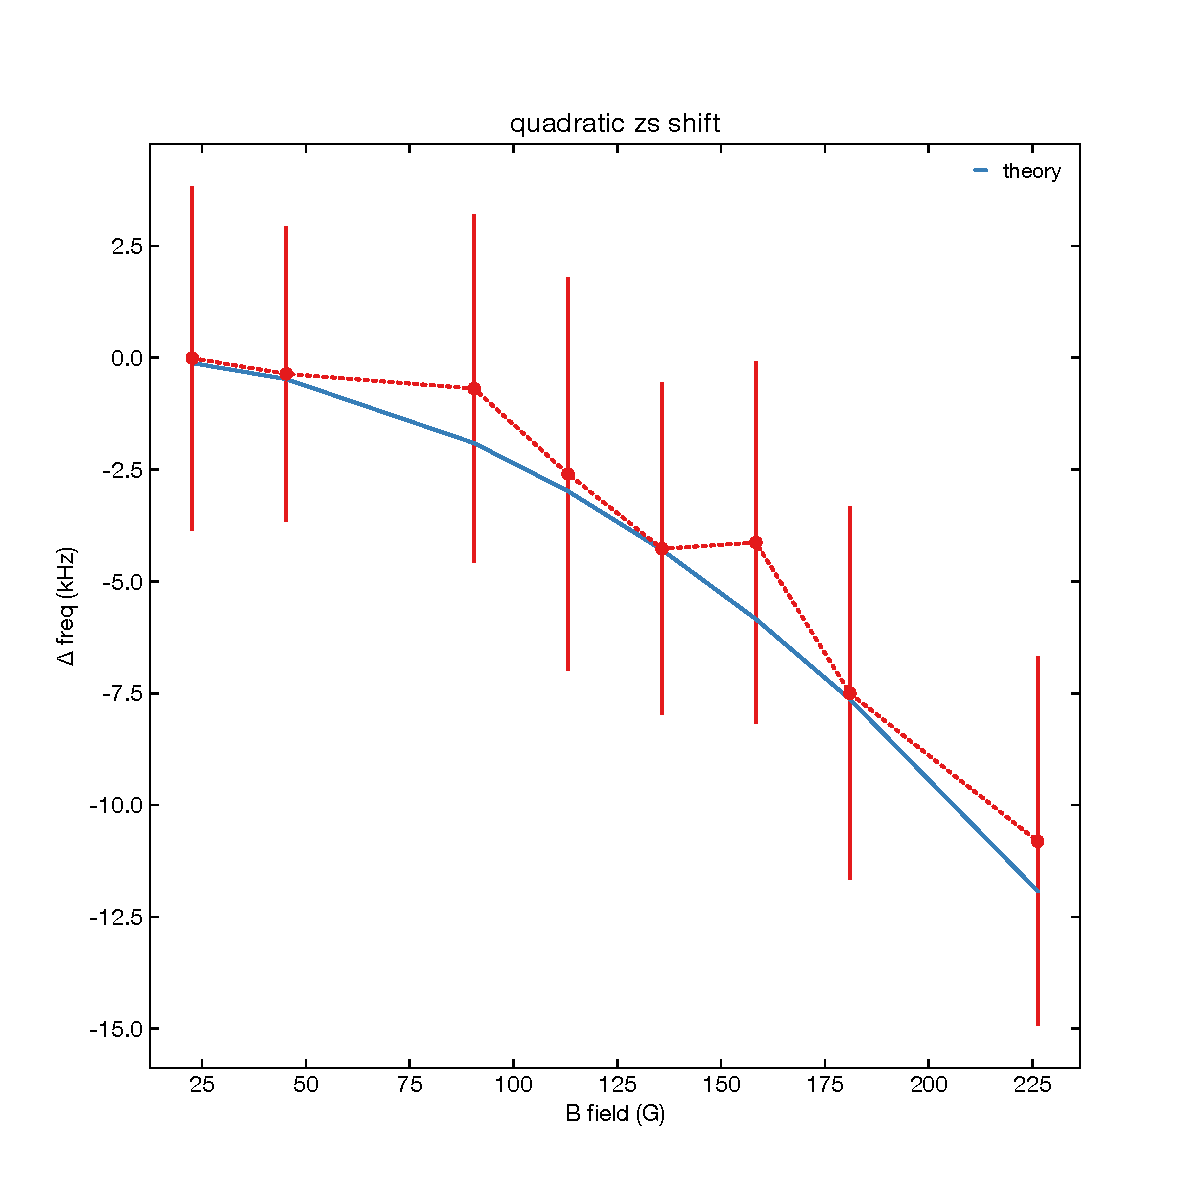
\includegraphics[scale=0.4]{figures/quadratic_zeeman_shift.pdf}
		    \caption{Quadratic zeeman shift}
		\end{subfigure}
		\caption{}
		\end{figure}


		% \begin{figure}
		% % \centering 
		% \hspace*{-2cm}
		% \label{fig:pol_ratio}
		% \begin{subfigure}{0.4\linewidth}
		% 	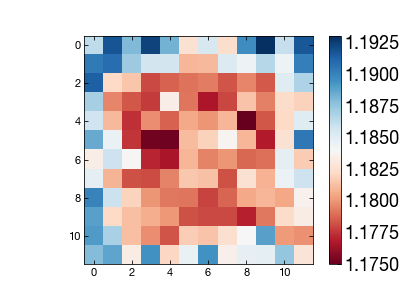
\includegraphics[scale=0.7]{figures/pol_ratio_size6.png}
		% 	% \caption{}
		% \end{subfigure}
		% \qquad\qquad\qquad\quad
		% \begin{subfigure}{0.4\linewidth}
		% 	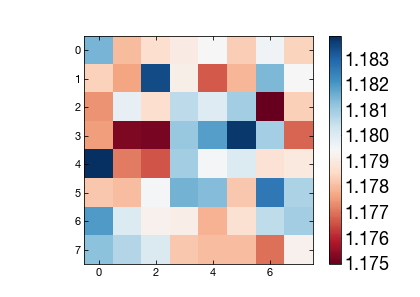
\includegraphics[scale=0.7]{figures/pol_ratio_size4.png}
		% 	% \caption{}
		% \end{subfigure}
		% \caption{Polarizability $\alpha_g/\alpha_e$ ratio for (a) larger size (b) smaller size} 
		% \end{figure}

			% \begin{figure}
			% \centering 
			% \begin{subfigure}[b]{0.4\linewidth}
			% 	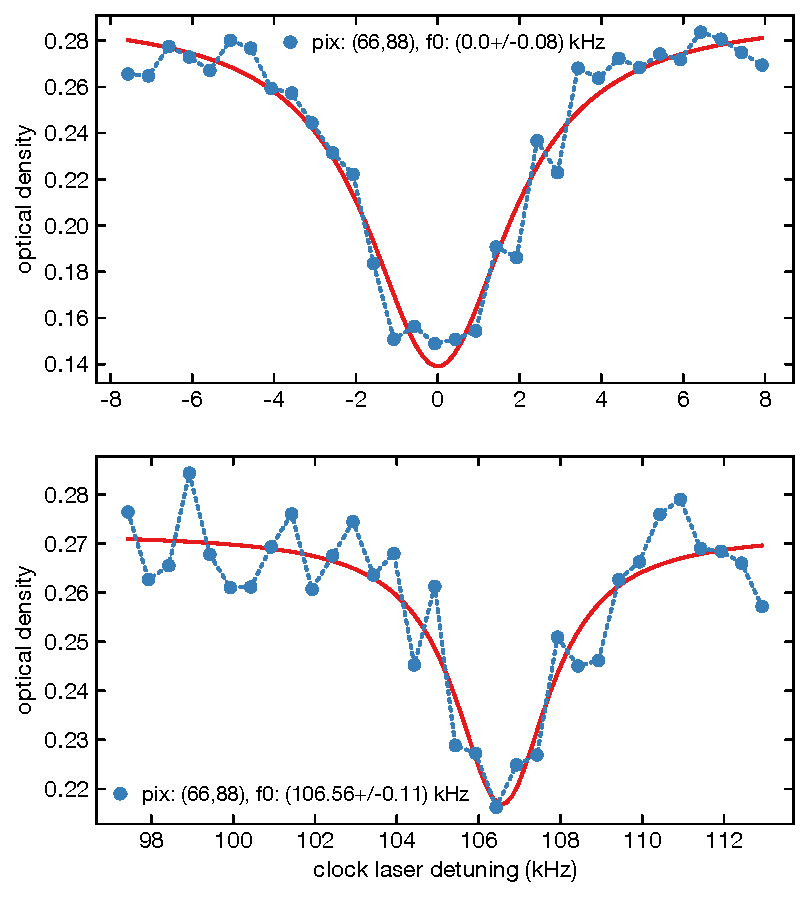
\includegraphics[scale=0.5]{figures/high_depth66_88.pdf}
			% 	\caption{}
			% \end{subfigure}
			% \qquad\qquad
			% \begin{subfigure}[b]{0.4\linewidth}
			% 	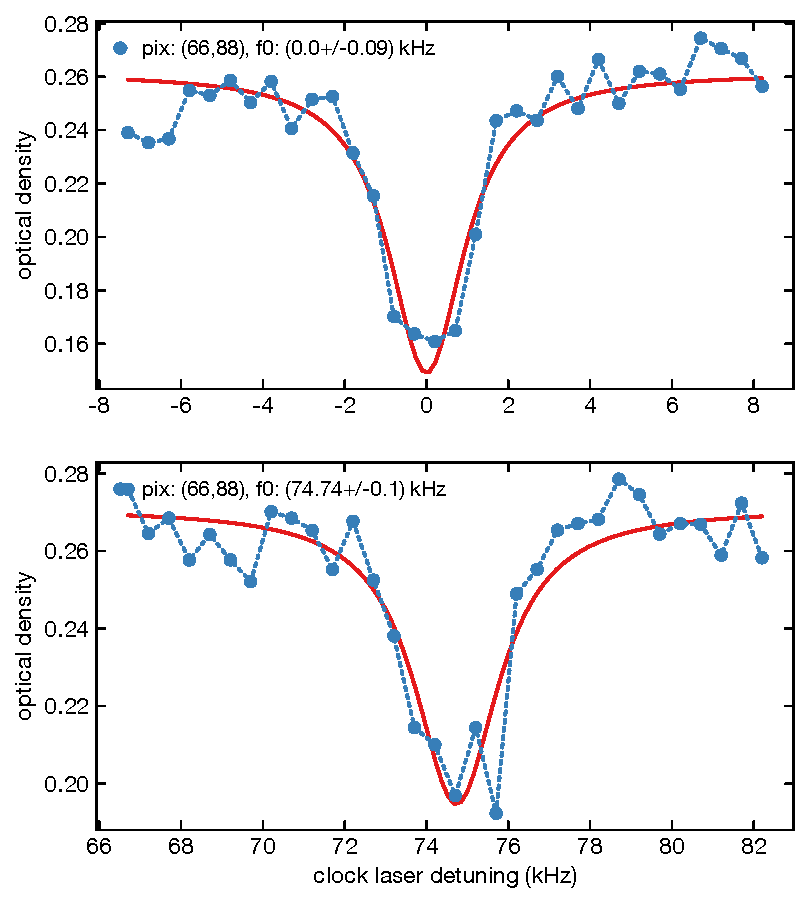
\includegraphics[scale=0.5]{figures/half_depth66_88.pdf}
			% 	\caption{}
			% \end{subfigure}

			% \begin{subfigure}{\linewidth}
			% 	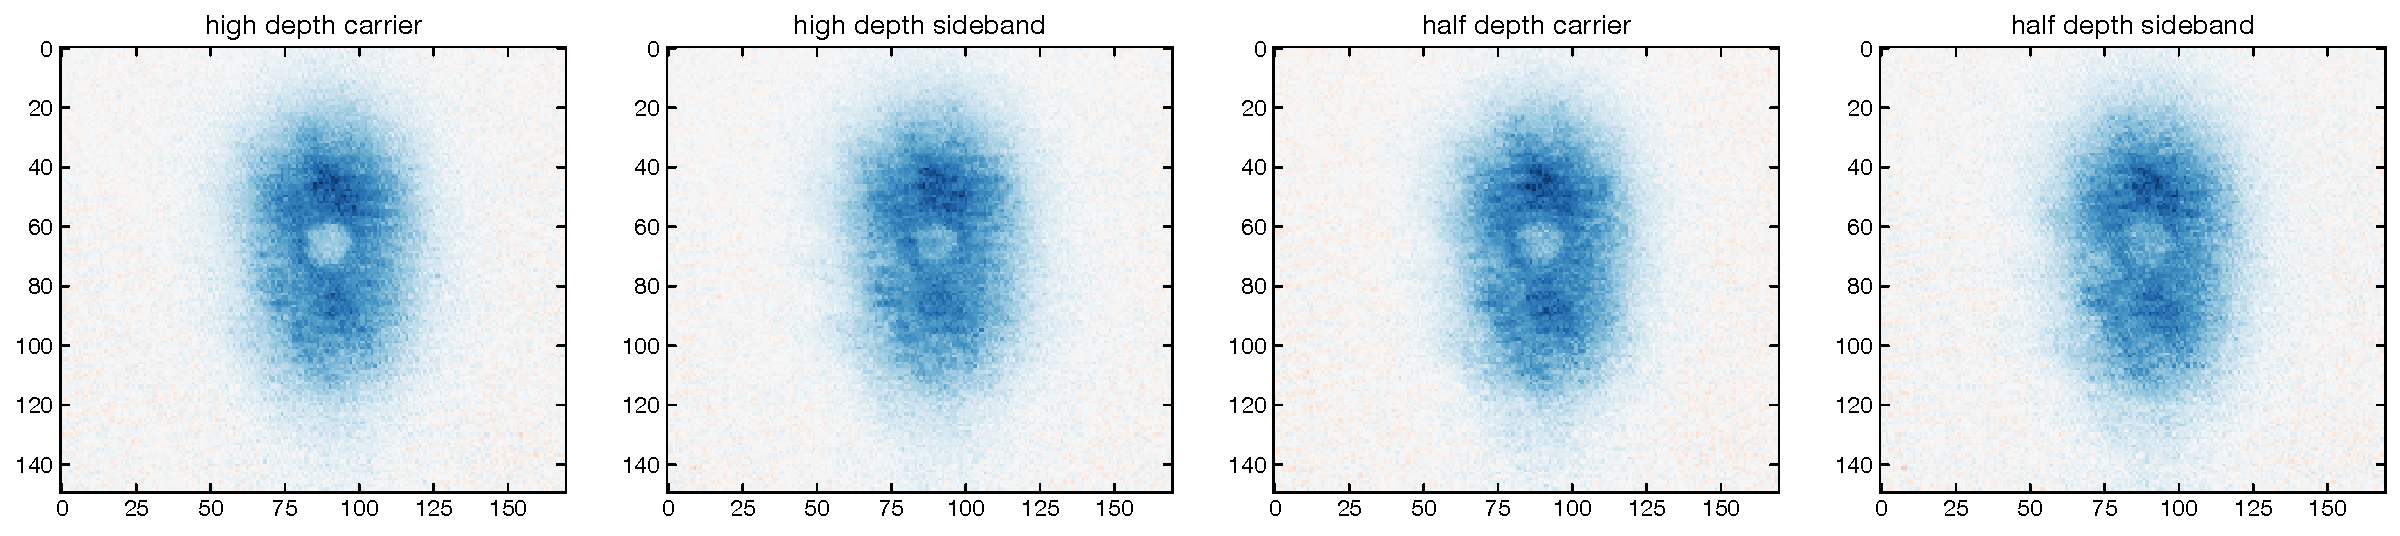
\includegraphics[scale=0.4]{figures/insitu_images.pdf}
			% 	\caption{}
			% \end{subfigure}
			% \caption{\textbf{(a)} carrier (top) and sideband (bottom) clock spectra of ground and excited states of high depth \textbf{(b)} same as (a) for half of the depth \textbf{(c)} in-situ \SSZ images at the center frequency of carrier and sideband spectra (data folder: \textbackslash data \textbackslash\_2020\textbackslash12\textbackslash02\textbackslash it\_sr88\_absolute\_ac\_stark)} 
			% \label{fig:total_ac_stark_spectrum}

			% \end{figure}


\subsection{Ac-Stark shift from the clock laser}
	very small
% \subsection{Magnetic field calibration}
% \subsection{Probe intensity calibration}

\bibliography{main}{}
\bibliographystyle{plain}
